\documentclass{article}
\usepackage{graphicx}
\usepackage{amsmath}
\renewcommand{\baselinestretch}{1}
\setlength{\textheight}{9in}
\setlength{\textwidth}{6.5in}
\setlength{\headheight}{0in}
\setlength{\headsep}{0in}
\setlength{\topmargin}{0in}
\setlength{\oddsidemargin}{0in}
\setlength{\evensidemargin}{0in}
\setlength{\parindent}{.3in}
\graphicspath{{images/}}

\title{Communication Systems \\
    \large Chapter 2 Signals and Signal Space}
\author{Hunter Mills}
\date{\today}

\begin{document}
    \maketitle

    \medskip
    Chapter 2 Signals and Signal Space is a review on signals and systems. 
    
    \section{Size of a Signal}
    Two common measures of signal strength are energy and signal power.

    \subsection{Signal Energy}
    The energy in a signal $g(t)$ the energy dissipated by $g(t)$ on a 1 Ohm resistor. 
    
    \begin{equation}  
        E_g = \int_{-\infty}^{\infty}g^2(t)dt
    \end{equation}
    which can be generalized to a complex signal with

    \begin{equation}
        E_g = \int_{-\infty}^{\infty}|g(t)|^2dt
    \end{equation}

    \subsection{Signal Power}
    Since some classes of signals can have infinite energy then it is not an adequate measure all the time. When the amplitude of $g(t)$ does not $\rightarrow 0$ as
    $t \rightarrow \infty$ then the signal energy will be infinite. The average power of a signal is

    \begin{equation}
        P_g = \lim_{T \rightarrow \infty} \frac{1}{T} \int_{-T/2}^{T/2} |g(t)|^2dt
    \end{equation}
    whereas the power in a period of a waveform is

    \begin{equation}
        P_g = \frac{1}{T} \int_{-T/2}^{T/2} |g(t)|^2dt
    \end{equation}

    \subsection{Units of Signal Energy and Power}
    The unit of signal energy and power are the joule (J) and the watt (W) respectively. In a logarithmic scale the signal power can be converted with

    \begin{equation}
        [10 * \log_{10} P] \textrm{dBw or} [30 + 10 * \log_{10} P] \textrm{dBm}
    \end{equation}
    For example -30 dBm corresponds to a signal power of $10^{-6}$ W in linear scale.

    \section{Classification of Signals}
    \begin{itemize}
        \item Continuous time and discrete time signals.
        \item Analog and digital signals.
        \item Periodic and aperiodic signals.
        \item Energy and power signals.
        \item Deterministic and random signals
    \end{itemize}

    \subsection{CT, DT, Analog and Digital Signals}
    A signal which is specified for every value of $t$ is a continuous signal where if a signal is only defined at $t = nT$ then it is discrete time. Along with these
    a analog signal can be any amplitude whereas a digital signal can only be a finite number of values.

    \subsection{Periodic and Aperiodic Signals}
    A signal $g(t)$ is \textbf{periodic} if there is a positive constant $T_0$ such that
    \begin{equation}
        g(t) = g(t + T_0) \quad \textrm{for all t}
    \end{equation}
    The smallest value of $T_0$ that satisfies the periodicity condition is the \textbf{period} of $g(t)$. If there is no $T_0$ that satisfies the condition
    then the signal is \textbf{aperiodic}.

    \subsection{Energy and Power Signals}
    A signal with finite energy is a \textbf{energy signal} and a signal with finite power is a \textbf{power signal}. A signal is an energy signal if
    \begin{equation}
        \int_{-\infty}^{\infty}|g(t)|^2dt < \infty
    \end{equation}
    and a power signal if
    \begin{equation}
        0 < \lim_{T \rightarrow \infty} \frac{1}{T} \int_{-T/2}^{T/2} |g(t)|^2dt < \infty
    \end{equation}
    A signal cannot be both a power and energy signal but a signal can be neither (a signal with infinite power eg. $g(t) = t$).

    \subsection{Deterministic and Random Signals}
    A signal whose physical description if known completely is a \textbf{deterministic signal} whereas a signal that only has some parts known is a 
    \textbf{random signal}.

    \section{Signal Operations}
    \subsection{Time Shifting}
    Consider a signal $g(t)$ and the same signal delayed by $T$ seconds $\phi (t)$. Whatever happens to $g(t)$ at some instant $t$ also happens in $\phi(t)$
    $T$ seconds later.
    \begin{equation}
        \phi (t + T) = g(t) 
    \end{equation}
    or 
    \begin{equation}
        \phi(t) = g(t-T)
    \end{equation}
    To time shift a signal by $T$ we replace $t$ with $t=T$. 

    \subsection{Time Scaling}
    The compression or expansion of a signal is called time scaling. To compress a signal by a factor of $a$ is done with
    \begin{equation}
        \phi (t) = g(at)
    \end{equation}
    and to expand a signal by a factor of $a$ is
    \begin{equation}
        \phi(t) = g(\frac{t}{a})
    \end{equation}

    \subsection{Time Inversion (Folding)}
    Time inversion can be considered a special case of time scaling with $a = -1$. This rotates the signal $180 \deg$ about $t = 0$. 

    \section{Unit Impulse Signal (Delta Function)}
    One of the most useful signals is the \textbf{Unit Impulse signal} ($\delta(t)$). The formulas that describe the unit impulse signal are
    \begin{equation}
        \delta (t) = 0 \textrm{ when } t \neq 0
    \end{equation}
    \begin{equation}
        \delta (t) = 1 \textrm{ when } t = 0
    \end{equation}
    \begin{equation}
        \int \delta (t)dt = 1
    \end{equation}

    \begin{figure}[h]
        \centering
        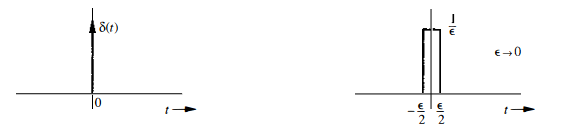
\includegraphics[width=0.75\textwidth]{delta}
        \caption{Unit Impulse and its approximation}
    \end{figure}

    \subsection{Multiplication of a Function by an Impulse}
    \begin{equation}
        \phi (t) \delta(t) = \phi (0) \delta(t)
    \end{equation}
    \begin{equation}
        \phi (t) \delta(t-T) = \phi (T) \delta(t-T)
    \end{equation}

    \subsection{Sampling Property of the Unit Impulse Function}
    \begin{equation}
        \int \phi(t) \delta (t-T)dt = \phi (T) \int \delta (t-T)dt = \phi (T)
    \end{equation}
    This equation is known as the \textbf{Sifting Property}.

    \section{The Unit Step Function $u(t)$}
    Another useful function if the \textbf{Unit Step Function}.
    \begin{equation}
        u(t) = 
        \begin{cases}
            1 \quad t \geq 0 \\
            0 \quad t < 0
        \end{cases}
    \end{equation}

    This can create a \textbf{causal signal}, a signal that starts after $t = 0$. The relationship between $u(t)$ and $\delta(t)$ can be shown with the 
    following two equations.

    \begin{equation}
        \int_{-\infty}^{t} \delta (\tau) d\tau = 
        \begin{cases}
            0 \quad t < 0 \\
            1 \quad t \geq 0
        \end{cases}
    \end{equation}

    \begin{equation}
        \frac{du}{dt} = \delta(t)
    \end{equation}

    \begin{figure}[h]
        \centering
        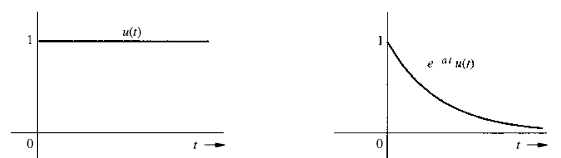
\includegraphics[width=0.75\textwidth]{step}
        \caption{$u(t)$ and $e^{-at}u(t)$}
    \end{figure}

    \section{Signals vs Vectors}
    Discrete signals can be represented as a vector with dimension $N$ over a closed interval. A signal vector $\textbf{g}$ of length $N$ can be described as
    \begin{equation}
        \textbf{g} = \left[g(t_0), g(t_2) \quad \textrm{...} \quad g(t_{N-1}) \right]
    \end{equation}
    A continuous time signal $g(t)$ can be written as
    \begin{equation}
        \lim_{N \rightarrow \infty} \textbf{g} = g(t) \quad \textrm{over the closed interval}
    \end{equation}
    This shows that basic definitions and operations in a Euclidean vector space can be applied to continuous time signals. $\textbf{x}$ is a vector with a
    magnitude $||\textbf{x}||$. The inner (dot or scalar) product of $\textbf{x}$ and $\textbf{g}$ is
    \begin{equation}
        <\textbf{g}, \textbf{x}> = ||\textbf{g}|| * ||\textbf{x}|| \cos \theta
    \end{equation}
    where $\theta$ is the angle between the two vectors. We can express $||\textbf{x}||$, the length (norm) of a vector $\textbf{x}$ as
    \begin{equation}
        ||\textbf{x}||^2=<\textbf{x}, \textbf{x}>
    \end{equation}

    \begin{figure}[h]
        \centering
        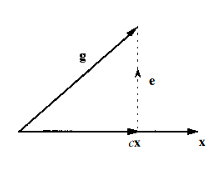
\includegraphics[width=0.75\textwidth]{vec}
        \caption{Projection of a vector along another vector}
    \end{figure}

    \subsection{Component of a Vector along Another Vector}
    The component of $\textbf{g}$ along $\textbf{x}$ is $c\textbf{x}$. The component of $\textbf{g}$ along $\textbf{x}$ is the projection of
    $\textbf{g}$ on the vector $\textbf{x}$ and is obtained by drawing a perpendicular vector from the tip of $\textbf{g}$ on the vector $\textbf{x}$. 
    \begin{equation}
        \textbf{g} = c\textbf{x} + \textbf{e}
    \end{equation}
    where $\textbf{e}$ is the error vector. If our goal is the approximate $\textbf{g}$ by $c\textbf{x}$ then the error in this approximation is 
    $\textbf{e} = \textbf{g} - c\textbf{x}$. The projection of a vector $\textbf{g}$ along $\textbf{x}$ is $c\textbf{x}$ where $c$ is choses to 
    minimize the norm of the error vector.

    \begin{figure}[h]
        \centering
        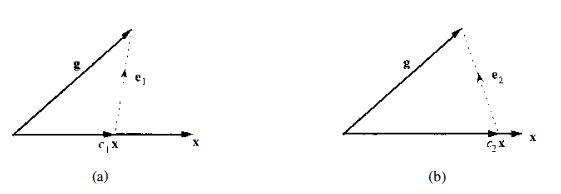
\includegraphics[width=0.75\textwidth]{proj}
        \caption{Approximations of a vector in terms of another vector}
    \end{figure}

    \begin{equation}
        c = \frac{<\textbf{g}, \textbf{x}>}{<\textbf{x}, \textbf{x}>} = \frac{1}{||\textbf{x}||^2}<\textbf{g}, \textbf{x}>
    \end{equation}

    \subsection{Signal Decomposition and Signal Components}
    If a signal $g(t)$ is approximated by another signal $x(t)$ as
    \begin{equation}
        g(t) \approx cx(t)
    \end{equation}
    then the optimum value $c$ that minimizes the energy of the error signal is
    \begin{equation}
        c = \frac{\int_{t_1}^{t_2}g(t)x(t)dt}{\int_{t_1}^{t_2}x^2(t)dt} = \frac{1}{E_x}\int_{t_1}^{t_2}g(t)x(t)dt
    \end{equation}
    If the component of a signal $g(t)$ of the form $x(t)$ is zero then the two signals are orthogonal. 
    \begin{equation}
        \int_{t_1}^{t_2}g(t)x(t)dt = 0
    \end{equation}
    The inner product of two (real) signals are
    \begin{equation}
        <g(t), x(t)> = \int_{t_1}^{t_2}g(t)x(t)dt
    \end{equation}
    The norm of a signal is
    \begin{equation}
        ||g(t)|| = \sqrt{<g(t), g(t)>}
    \end{equation}

    \subsection{Complex Signal Space and Orthogonality}
    To approximate a complex signal g(t) by a function x(t) as 
    \begin{equation}
        g(t) \approx cx(t)
    \end{equation}
    the optimum $c$ is defined as
    \begin{equation}
        c = \frac{1}{E_x}\int_{t_1}^{t_2}g(t)x^\ast(t)dt
    \end{equation}
    Complex signals are orthogonal if
    \begin{equation}
        \int_{t_1}^{t_2}x_1(t)x_2^\ast(t)dt = 0 \quad \textrm{or} \quad \int_{t_1}^{t_2}x_1^\ast(t)x_2(t)dt = 0
    \end{equation}

    \subsection{Energy of the Sum of orthogonal signals}
    If signals $x(t)$ and $y(t)$ are orthogonal over the interval $[t_1, t_2]$ and if $z(t) = x(t) + y(t)$ then
    \begin{equation}
        E_z = E_x + E_y
    \end{equation}
    and 
    \begin{equation}
        \int_{t_1}^{t_2}|x(t) + y(t)|^2dt = \int_{t_1}^{t_2}|x(t)|^2dt + \int_{t_1}^{t_2}|y(t)|^2dt
    \end{equation}

    \section{Correlation of Signals}
    Similarity between two vectors is indicated by the angle $\theta$ between the vectors. The smaller the $\theta$ the larger the similarity. The \textbf{
    correlation coefficient} $\rho$ is defined as
    \begin{equation}
        \rho = \cos \theta = \frac{<\textbf{g}, \textbf{x}>}{||\textbf{g}|| ||\textbf{x}||}
    \end{equation}
    where the magnitude of $\rho$ will never be greater than 1. If the two vectors are aligned then $\rho = 1$ whereas if the vectors or orthogonal then 
    $\rho = 0$. To convert that to signals the \textbf{correlation coefficient, $\rho$} will be
    \begin{equation}
        \rho = \frac{1}{\sqrt{E_gE_x}}\int_{-\infty}^{\infty}g(t)x(t)dt
    \end{equation}
    When $g(t) = kx(t)$ then $\rho = 1$, $g(t) = -kx(t)$ then $\rho = -1$ and when the signals are orthogonal then $\rho = 0$. For complex signals
    \begin{equation}
        \rho = \frac{1}{\sqrt{E_gE_x}}\int_{-\infty}^{\infty}g(t)x^*(t)dt
    \end{equation}

    \subsection{Correlation Functions}
    A transmitted pulse $g(t)$ and a received pulse $z(t)$ are shown in the next figure. 

    \begin{figure}[h]
        \centering
        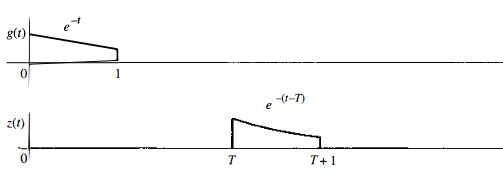
\includegraphics[width=0.75\textwidth]{corr}
        \caption{Radar Pulse}
    \end{figure}

    Since in time the integral for the correlation coefficient is
    \begin{equation}
        \rho = \frac{1}{\sqrt{E_gE_x}}\int_{-\infty}^{\infty}z(t)g^*(t)dt = 0
    \end{equation}
    it shows that the signals are orthogonal when they are clearly the same signal time shifted. To fix this issue, we can use \textbf{cross correlation} 
    which is defined as
    \begin{equation}
        \psi_{zg}(\tau) = \int_{-\infty}^{\infty}z(t)g^*(t-\tau)dt = \int_{-\infty}^{\infty}z(t + \tau)g^*(t)dt
    \end{equation}
    If for some value of $\tau$ there is a strong correlation, we can find the presence of a pulse and also the relative time shift of $z(t)$. 

    \subsection{Autocorrelation Function}
    The correlation of a signal with itself is called \textbf{autocorrelation}. The autocorrelation function of a real signal $g(t)$ is defined as
    \begin{equation}
        \psi_{g}(\tau) = \int_{-\infty}^{\infty}g(t)g(t+\tau)dt
    \end{equation}
    This measures the similarity of $g(t)$ with its displaced self.  

    \section{Trigonometric Fourier Series}
    A signal $g(t)$ can be expressed by the Trigonometric Fourier series over the interval $[t_1, t_1+T_0]$ as 
    \begin{equation}
        g(t) = a_0 + \sum_{n=1}^{\infty}(a_n \cos n \omega_0 t + b_n \sin n \omega_0 t) \quad t_1 \leq t \leq t_1+T_0
    \end{equation}
    where 
    \begin{eqnarray}
        \omega_0 = 2\pi f_0 = \frac{2\pi}{T_0} \quad \textrm{and} \quad f_0 = \frac{1}{T_0}
    \end{eqnarray}
    The coefficients can be described as
    \begin{equation}
        a_0 = \frac{1}{T_0}\int_{t_1}^{t_1+T_0} g(t)dt
    \end{equation}
    \begin{equation}
        a_n = \frac{2}{T_0}\int_{t_1}^{t_1+T_0} g(t)\cos n\omega_0tdt \quad n=1,2,3...
    \end{equation}
    and 
    \begin{equation}
        b_n = \frac{2}{T_0}\int_{t_1}^{t_1+T_0} g(t)\sin n\omega_0tdt \quad n=1,2,3...
    \end{equation}
    If $g(t)$ is periodic with $T_0$ then 
    \begin{equation}
        g(t) = a_0 + \sum_{n=1}^{\infty}(a_n \cos n \omega_0 t + b_n \sin n \omega_0 t) \quad \textrm{for all } t
    \end{equation}
    If $g(t)$ is real then the \textbf{Compact Trigonometric Fourier Series} is defined as
    \begin{equation}
        g(t) = C_0 + \sum_{n=1}^{\infty}(C_n \cos (2n\pi f_0 t + \theta_n) \quad \textrm{for all } t
    \end{equation}
    where
    \begin{equation}
        C_n = \sqrt{a_n^2 + b_n^2}
    \end{equation}
    \begin{equation}
        \theta_n = \tan^{-1}()\frac{-b_n}{a_n})
    \end{equation}
    and $C_0 = a_0$.

    \subsection{Finding Trigonometric Fourier Series for Aperiodic Signals}
    $\varphi(t)$ is the periodic extension of $g(t)$. The fourier series $g(t)$ over a interval of $T_0$ and the fourier series $\varphi(t)$ need only be
    equal over that interval of $T_0$.
    \begin{equation}
        a_0 = \frac{1}{T_0}\int_{t_0} g(t)dt
    \end{equation}
    \begin{equation}
        a_n = \frac{2}{T_0}\int_{t_0} g(t)\cos n\omega_0tdt \quad n=1,2,3...
    \end{equation}
    and 
    \begin{equation}
        b_n = \frac{2}{T_0}\int_{t_0} g(t)\sin n\omega_0tdt \quad n=1,2,3...
    \end{equation}

    \subsection{Existence of the Fourier Series: Dirichlet Conditions}
    For the series to exist then the coefficients $a_0$, $a_n$ and $b_n$ must be finite.
    \begin{equation}
        \int_{T_0}|g(t)|dt < 0
    \end{equation}
    The \textbf{weak Dirichlet Condition} (above) says that if a periodic function $g(t)$ satisfies the weak Dirichlet Condition then the fourier series
    exists but may not converge at every point. \\
    The other condition that must be true is that the number of maxima and minima in one period are finite and the number of discontinuities are finite. Both
    these conditions make up the \textbf{strong Dirichlet Conditions}.

    \subsection{Exponential Fourier Series}
    Recall that
    \begin{equation}
        e^{j2\pi f_0t} = \cos(2\pi f_0t) + j\sin(2\pi f_0 t)
    \end{equation}
    From this relation we can create a slightly different series expansion called the \textbf{Exponential Fourier Series}.
    \begin{equation}
        x(t) = \sum_{n=-\infty}^{\infty}c_n e^{j2\pi nf_0t} \quad 0 < t < T_0
    \end{equation}
    where 
    \begin{equation}
        c_n = \frac{1}{T_0}\int_{0}^{T_0}x(t)e^{-j2\pi n f_0t}dt
    \end{equation}

    \subsection{The Fourier Spectrum}
    Check notes on DSP for this description (CH4).

    \end{document}